% ============================================================
% DEPENDÊNCIAS DESTE CAPÍTULO
%
% Adicionar ao preâmbulo do documento principal, caso ainda
% não estejam presentes:
%
% \usepackage{booktabs}
% \usepackage{longtable}
% \usepackage{float}
% \usepackage{tikz}
% \usepackage{pgfplots}
%
% \usetikzlibrary{
%     arrows.meta,
%     positioning,
%     shapes.geometric
% }
%
% \pgfplotsset{compat=1.18}
% ============================================================


\chapter{Atividade 1 -- Multiplicação matriz por vetor e acesso a memória}

\label{chap:atvd01}


% ============================================================
% ENUNCIADO
% ============================================================

\section{Enunciado da tarefa}

\label{sec:atvd01-enunciado}

\begin{quote}

Implemente duas versões da multiplicação de matriz por vetor (MxV) em C:
uma versão com acesso a matriz por linhas, utilizando linha externa e
coluna interna; outra versão com acesso a matriz por colunas, utilizando
coluna externa e linha interna.

Meça o tempo de execução de cada versão utilizando uma função apropriada
de temporização e execute testes com diferentes tamanhos de matriz.

Identifique a partir de que tamanho os tempos das duas implementações
passam a divergir significativamente e explique por que isso ocorre,
relacionando as observações com o uso da memória cache e o padrão de
acesso a memória.

\end{quote}


% ============================================================
% OBJETIVOS
% ============================================================

\section{Objetivos e requisitos}

\label{sec:atvd01-objetivos}

A atividade tem como objetivo avaliar experimentalmente o impacto do
padrão de acesso à memória sobre o desempenho da multiplicação
matriz-vetor.

As duas implementações executam a mesma operação matemática e possuem a
mesma complexidade assintótica, diferindo essencialmente na ordem em que
os elementos da matriz são percorridos.

Os principais requisitos identificados para o experimento são:

\begin{itemize}

    \item implementar a multiplicação matriz-vetor com percurso da matriz
    por linhas;

    \item implementar a mesma operação com percurso da matriz por colunas;

    \item utilizar a mesma representação de dados nas duas versões;

    \item variar sistematicamente a dimensão da matriz;

    \item medir exclusivamente o trecho correspondente à multiplicação;

    \item utilizar uma fonte de tempo monotônica;

    \item realizar múltiplas medições para reduzir a influência de ruído
    experimental;

    \item validar a equivalência funcional entre as duas implementações;

    \item apresentar os tempos de forma comparável;

    \item calcular uma métrica adicional que represente diretamente a
    diferença entre os dois padrões de acesso;

    \item relacionar os resultados obtidos com localidade espacial,
    stride de memória e hierarquia de cache.

\end{itemize}

Como métrica comparativa adicional foi definida a razão:

\begin{equation}
    C/L =
    \frac{T_{\mathrm{coluna}}}
         {T_{\mathrm{linha}}},
    \label{eq:atvd01-cl}
\end{equation}

em que \(T_{\mathrm{coluna}}\) representa o tempo da implementação com
percurso por colunas e \(T_{\mathrm{linha}}\) representa o tempo da
implementação com percurso por linhas.

A interpretação da métrica é direta:

\begin{itemize}

    \item \(C/L \approx 1\): tempos semelhantes;

    \item \(C/L > 1\): a versão por colunas apresenta maior tempo;

    \item \(C/L < 1\): a versão por colunas apresenta menor tempo na
    medição considerada.

\end{itemize}


% ============================================================
% FUNDAMENTAÇÃO
% ============================================================

\section{Fundamentação conceitual}

\label{sec:atvd01-fundamentacao}

\subsection{Multiplicação matriz-vetor}

Considere uma matriz quadrada \(A\) de dimensão \(N \times N\), um vetor
\(x\) com \(N\) elementos e um vetor resultado \(y\).

A multiplicação matriz-vetor é definida por:

\begin{equation}
    y_i =
    \sum_{j=0}^{N-1}
    A_{ij}x_j,
    \qquad
    i = 0,1,\ldots,N-1.
    \label{eq:atvd01-mxv}
\end{equation}

Para cada posição do vetor de saída é calculado o produto interno entre
uma linha da matriz e o vetor de entrada.

As duas implementações avaliadas realizam aproximadamente \(N^2\)
multiplicações e \(N^2\) acumulações. Portanto, ambas apresentam
complexidade assintótica:

\begin{equation}
    O(N^2).
\end{equation}

A atividade não compara algoritmos com ordens de complexidade distintas.
O aspecto central é a diferença entre os padrões de acesso aos dados.


\subsection{Organização row-major}

Na representação utilizada pelo programa, a matriz é armazenada em um
único bloco contínuo de memória.

O elemento lógico:

\begin{equation}
    A[i][j]
\end{equation}

é acessado por:

\begin{equation}
    A[i \times N + j].
    \label{eq:atvd01-rowmajor}
\end{equation}

Essa representação corresponde à organização \textit{row-major}, em que
os elementos pertencentes a uma mesma linha ocupam posições consecutivas
na memória.

Assim, a sequência:

\begin{verbatim}
A[i][0], A[i][1], A[i][2], ...
\end{verbatim}

corresponde a acessos contíguos.

Por outro lado, a sequência:

\begin{verbatim}
A[0][j], A[1][j], A[2][j], ...
\end{verbatim}

realiza saltos entre posições pertencentes a linhas diferentes.


\subsection{Localidade espacial}

A hierarquia de memória transfere dados em blocos, e não necessariamente
um elemento isolado por acesso.

Quando um programa utiliza uma posição de memória, elementos próximos
também podem ser disponibilizados em níveis rápidos da hierarquia.

O percurso por linhas explora esse comportamento porque os elementos
subsequentes da linha estão armazenados em posições adjacentes.

Esse comportamento é associado à \textbf{localidade espacial}.


\subsection{Stride de memória}

O \textit{stride} representa a distância, em bytes, entre endereços
sucessivos acessados por uma determinada sequência de execução.

Na implementação por linhas, utilizando dados do tipo \texttt{int}, o
stride principal sobre a matriz é aproximadamente:

\begin{equation}
    S_{\mathrm{linha}} = sizeof(int).
\end{equation}

No ambiente utilizado:

\begin{equation}
    sizeof(int) = 4\ \text{bytes}.
\end{equation}

Portanto:

\begin{equation}
    S_{\mathrm{linha}} = 4\ \text{bytes}.
\end{equation}

Na implementação por colunas:

\begin{equation}
    S_{\mathrm{coluna}}
    =
    N \times sizeof(int).
    \label{eq:atvd01-stride}
\end{equation}

Por exemplo, para \(N=2000\):

\begin{equation}
    S_{\mathrm{coluna}}
    =
    2000 \times 4
    =
    8000\ \text{bytes}.
\end{equation}

Para \(N=5000\):

\begin{equation}
    S_{\mathrm{coluna}}
    =
    5000 \times 4
    =
    20000\ \text{bytes}.
\end{equation}

O aumento do stride reduz a capacidade de aproveitar imediatamente os
dados vizinhos carregados pela hierarquia de memória.


\subsection{Hierarquia de memória}

O desempenho observado depende da interação entre o padrão de acesso e
a hierarquia de memória:

\begin{verbatim}
Registradores
     |
Cache L1
     |
Cache L2
     |
Cache L3
     |
Memória principal
\end{verbatim}

Os níveis mais próximos do processador apresentam menor capacidade, mas
menor latência.

Conforme o conjunto de dados aumenta, uma parcela crescente dos acessos
pode depender de níveis mais distantes da hierarquia.

Entretanto, o tamanho nominal de uma cache não constitui, isoladamente,
um limiar rígido de desempenho. Associatividade, políticas de
substituição, prefetching, tradução de endereços e os demais dados
utilizados pelo programa também influenciam o comportamento observado.


% ============================================================
% INTERPRETAÇÃO DIDÁTICA
% ============================================================

\section{Interpretação didática da tarefa}

\label{sec:atvd01-interpretacao}

O aspecto didático central da atividade é demonstrar que a complexidade
assintótica não caracteriza sozinha o desempenho real de uma
implementação.

As duas versões executam a mesma multiplicação e possuem complexidade
\(O(N^2)\). Entretanto, a ordem dos laços modifica a sequência de
endereços acessados.

A versão por linhas apresenta o padrão:

\begin{verbatim}
A[0][0] -> A[0][1] -> A[0][2] -> ...
\end{verbatim}

enquanto a versão por colunas apresenta:

\begin{verbatim}
A[0][0] -> A[1][0] -> A[2][0] -> ...
\end{verbatim}

A primeira acompanha a organização física dos dados em memória. A segunda
introduz um stride proporcional a \(N\).

A atividade permite, portanto, estabelecer a relação:

\begin{equation}
\text{ordem dos laços}
\rightarrow
\text{padrão de acesso}
\rightarrow
\text{localidade}
\rightarrow
\text{comportamento da cache}
\rightarrow
\text{tempo de execução}.
\end{equation}


% ============================================================
% MODELAGEM
% ============================================================

\section{Modelagem da solução}

\label{sec:atvd01-modelagem}

\subsection{Estrutura geral}

O experimento foi estruturado como um benchmark controlado.

Para cada dimensão \(N\), são realizadas as seguintes etapas:

\begin{enumerate}

    \item alocação da matriz e dos vetores;

    \item inicialização determinística dos dados;

    \item execução de aquecimento das duas implementações;

    \item validação inicial dos resultados;

    \item execução das medições válidas;

    \item cálculo da mediana dos tempos;

    \item cálculo da razão \(C/L\);

    \item apresentação dos resultados;

    \item liberação da memória.

\end{enumerate}

As dimensões avaliadas são:

\begin{equation}
    N =
    100,200,300,\ldots,5000.
\end{equation}

O intervalo de 100 permite acompanhar progressivamente o comportamento da
hierarquia de memória sem restringir o experimento a poucos pontos.


\subsection{Principais funções e componentes}

A implementação é organizada nos seguintes componentes:

\begin{description}

    \item[\texttt{inicializar\_dados()}]
    Inicializa a matriz e o vetor com valores inteiros determinísticos.

    \item[\texttt{mxv\_linhas()}]
    Executa a multiplicação utilizando linha externa e coluna interna.

    \item[\texttt{mxv\_colunas()}]
    Executa a multiplicação utilizando coluna externa e linha interna.

    \item[\texttt{tempo\_decorrido()}]
    Calcula o intervalo entre dois valores de
    \texttt{struct timespec}.

    \item[\texttt{medir\_linhas()}]
    Cronometra exclusivamente a execução do kernel por linhas.

    \item[\texttt{medir\_colunas()}]
    Cronometra exclusivamente a execução do kernel por colunas.

    \item[\texttt{calcular\_mediana()}]
    Determina a mediana das repetições válidas.

    \item[\texttt{validar\_resultados()}]
    Verifica a igualdade entre os vetores produzidos pelas duas versões.

    \item[\texttt{main()}]
    Controla a variação de \(N\), as repetições, as validações e a
    apresentação dos resultados.

\end{description}


% ============================================================
% DECISÕES
% ============================================================

\section{Decisões de projeto e trade-offs}

\label{sec:atvd01-decisoes}

\subsection{Uso do tipo inteiro}

A versão final do experimento utiliza dados do tipo \texttt{int}.

Essa decisão simplifica a implementação e permite validar as duas versões
por igualdade exata, sem a necessidade de tolerâncias numéricas próprias
de operações em ponto flutuante.

A inicialização utiliza valores reduzidos:

\begin{verbatim}
x[i] = (i % 5) + 1

A[i][j] = ((i + j) % 10) + 1
\end{verbatim}

Assim, mesmo no maior caso avaliado, o valor acumulado permanece dentro
da faixa de representação de um inteiro de 32 bits.

Um limite superior conservador é:

\begin{equation}
    5000 \times 10 \times 5
    =
    250000.
\end{equation}

O uso de \texttt{int} também reduz pela metade o volume da matriz em
relação a uma implementação equivalente com \texttt{double}. Por esse
motivo, resultados obtidos anteriormente com \texttt{double} não são
misturados ao conjunto experimental final.


\subsection{Representação contínua da matriz}

A matriz é alocada como um único vetor de \(N^2\) elementos.

Essa representação foi escolhida para:

\begin{itemize}

    \item garantir contiguidade física dos elementos;

    \item tornar explícita a organização row-major;

    \item evitar o overhead estrutural de um vetor de ponteiros;

    \item permitir que o stride seja derivado diretamente da expressão
    \(iN+j\).

\end{itemize}


\subsection{Mediana em vez da média}

Cada implementação é medida dez vezes para cada dimensão.

A mediana foi utilizada como estatística representativa por ser menos
sensível a medições excepcionalmente altas causadas por escalonamento do
sistema operacional, interrupções e outras interferências temporárias.


\subsection{Alternância da ordem de execução}

A ordem entre as versões por linhas e por colunas é alternada a cada
repetição.

Nas repetições pares:

\begin{verbatim}
linhas -> colunas
\end{verbatim}

e nas repetições ímpares:

\begin{verbatim}
colunas -> linhas
\end{verbatim}

Essa estratégia reduz o viés introduzido pela execução sistemática de
uma das versões antes da outra.


\subsection{Região cronometrada}

A alocação, a inicialização dos dados, a validação e a impressão dos
resultados permanecem fora da região cronometrada.

Na implementação por colunas, o vetor de saída precisa ser zerado antes
de cada execução devido ao uso de acumulações sucessivas. Essa operação
também é realizada fora da região medida.

Dessa forma, o tempo registrado corresponde diretamente ao kernel de
multiplicação.


\subsection{Otimização do compilador}

O programa foi compilado com \texttt{-O2}.

Esse nível permite avaliar uma implementação otimizada em condições
realistas, mantendo o mesmo conjunto de opções para ambas as versões.

Como consequência, transformações realizadas automaticamente pelo
compilador podem influenciar os tempos absolutos. Entretanto, as duas
implementações permanecem submetidas às mesmas condições de compilação.


% ============================================================
% DIAGRAMA ESTRUTURAL
% ============================================================

\section{Representação estrutural da implementação}

\label{sec:atvd01-estrutura}

A Figura~\ref{fig:atvd01-estrutura} apresenta os principais componentes
da implementação e suas relações.

\begin{figure}[H]
    \centering

    \tikzset{
        atvdblock/.style={
            draw,
            rounded corners,
            align=center,
            minimum width=4.0cm,
            minimum height=0.85cm
        },
        atvdarrow/.style={
            -{Latex[length=2.5mm]},
            thick
        }
    }

    \begin{tikzpicture}[
        node distance=1.0cm and 1.5cm
    ]

        \node[atvdblock] (main)
            {\texttt{main()}\\Controle do experimento};

        \node[atvdblock, below=of main] (dados)
            {Alocação e inicialização\\
             \texttt{inicializar\_dados()}};

        \node[atvdblock, below left=of dados] (linhas)
            {\texttt{mxv\_linhas()}\\
             Percurso contíguo};

        \node[atvdblock, below right=of dados] (colunas)
            {\texttt{mxv\_colunas()}\\
             Percurso com stride};

        \node[atvdblock, below=of linhas] (medirlinhas)
            {\texttt{medir\_linhas()}};

        \node[atvdblock, below=of colunas] (medircolunas)
            {\texttt{medir\_colunas()}};

        \node[atvdblock,
              below=2.0cm of $(medirlinhas)!0.5!(medircolunas)$]
              (validacao)
            {Validação dos resultados};

        \node[atvdblock, below=of validacao] (estatistica)
            {Mediana e razão \(C/L\)};

        \node[atvdblock, below=of estatistica] (saida)
            {Saída tabular no terminal};

        \draw[atvdarrow] (main) -- (dados);
        \draw[atvdarrow] (dados) -- (linhas);
        \draw[atvdarrow] (dados) -- (colunas);

        \draw[atvdarrow] (linhas) -- (medirlinhas);
        \draw[atvdarrow] (colunas) -- (medircolunas);

        \draw[atvdarrow] (medirlinhas) -- (validacao);
        \draw[atvdarrow] (medircolunas) -- (validacao);

        \draw[atvdarrow] (validacao) -- (estatistica);
        \draw[atvdarrow] (estatistica) -- (saida);

    \end{tikzpicture}

    \caption{Estrutura funcional do benchmark da Atividade 1.}
    \label{fig:atvd01-estrutura}

\end{figure}


% ============================================================
% FLUXO
% ============================================================

\section{Fluxo de execução}

\label{sec:atvd01-fluxo}

A Figura~\ref{fig:atvd01-fluxo} representa o fluxo executado para cada
valor de \(N\).

\begin{figure}[H]
    \centering

    \tikzset{
        flowblock/.style={
            draw,
            rounded corners,
            align=center,
            minimum width=5.3cm,
            minimum height=0.8cm
        },
        flowdecision/.style={
            draw,
            diamond,
            aspect=2.2,
            align=center,
            inner sep=1.5pt
        },
        flowarrow/.style={
            -{Latex[length=2.5mm]},
            thick
        }
    }

    \begin{tikzpicture}[
        node distance=0.75cm
    ]

        \node[flowblock] (inicio)
            {Seleciona dimensão \(N\)};

        \node[flowblock, below=of inicio] (aloca)
            {Aloca matriz e vetores};

        \node[flowblock, below=of aloca] (init)
            {Inicializa \(A\) e \(x\)};

        \node[flowblock, below=of init] (warm)
            {Executa warm-up das duas versões};

        \node[flowblock, below=of warm] (valini)
            {Validação inicial};

        \node[flowblock, below=of valini] (rep)
            {Executa 10 medições\\
             com ordem alternada};

        \node[flowblock, below=of rep] (valfim)
            {Validação final};

        \node[flowblock, below=of valfim] (mediana)
            {Calcula medianas e \(C/L\)};

        \node[flowblock, below=of mediana] (print)
            {Imprime resultado};

        \node[flowblock, below=of print] (free)
            {Libera memória};

        \node[flowdecision, below=1.0cm of free] (fim)
            {\(N < 5000\)?};

        \node[flowblock, below=1.0cm of fim] (encerra)
            {Fim};

        \draw[flowarrow] (inicio) -- (aloca);
        \draw[flowarrow] (aloca) -- (init);
        \draw[flowarrow] (init) -- (warm);
        \draw[flowarrow] (warm) -- (valini);
        \draw[flowarrow] (valini) -- (rep);
        \draw[flowarrow] (rep) -- (valfim);
        \draw[flowarrow] (valfim) -- (mediana);
        \draw[flowarrow] (mediana) -- (print);
        \draw[flowarrow] (print) -- (free);
        \draw[flowarrow] (free) -- (fim);

        \draw[flowarrow]
            (fim.east)
            -- ++(2.2,0)
            |- node[pos=0.15, right]{sim}
            (inicio.east);

        \draw[flowarrow]
            (fim)
            -- node[right]{não}
            (encerra);

    \end{tikzpicture}

    \caption{Fluxo experimental executado para cada dimensão da matriz.}
    \label{fig:atvd01-fluxo}

\end{figure}


% ============================================================
% METODOLOGIA
% ============================================================

\section{Metodologia experimental}

\label{sec:atvd01-metodologia}

\subsection{Ambiente de execução}

O experimento foi executado em uma máquina equipada com processador
Intel Core i7-14700K.

As informações de cache obtidas no sistema operacional foram:

\begin{table}[H]
    \centering

    \caption{Configuração de hardware considerada no experimento.}
    \label{tab:atvd01-hardware}

    \begin{tabular}{ll}
        \toprule
        \textbf{Característica}
        &
        \textbf{Valor}
        \\
        \midrule

        Processador
        &
        Intel Core i7-14700K
        \\

        Cache L2 total reportada
        &
        28672 KiB (28 MiB)
        \\

        Cache L3 reportada
        &
        33792 KiB (33 MiB)
        \\

        \bottomrule
    \end{tabular}

\end{table}

O valor de L2 apresentado corresponde ao total reportado pelo sistema e
não deve ser interpretado como uma única cache L2 compartilhada de
28 MiB disponível integralmente para uma thread.

O ambiente de software é apresentado na
Tabela~\ref{tab:atvd01-software}.

\begin{table}[H]
    \centering

    \caption{Configuração de software utilizada.}
    \label{tab:atvd01-software}

    \begin{tabular}{ll}
        \toprule
        \textbf{Característica}
        &
        \textbf{Configuração}
        \\
        \midrule

        Sistema
        &
        Windows
        \\

        Ambiente
        &
        MSYS2 UCRT64
        \\

        Compilador
        &
        GCC 15.1.0
        \\

        Linguagem
        &
        C
        \\

        Padrão
        &
        C11
        \\

        Otimização
        &
        \texttt{-O2}
        \\

        Relógio
        &
        \texttt{CLOCK\_MONOTONIC}
        \\

        Tipo principal
        &
        \texttt{int}
        \\

        \bottomrule
    \end{tabular}

\end{table}


\subsection{Configuração das medições}

Os parâmetros utilizados no benchmark são apresentados na
Tabela~\ref{tab:atvd01-parametros}.

\begin{table}[H]
    \centering

    \caption{Parâmetros experimentais da Atividade 1.}
    \label{tab:atvd01-parametros}

    \begin{tabular}{ll}
        \toprule
        \textbf{Parâmetro}
        &
        \textbf{Valor}
        \\
        \midrule

        \(N_{\min}\)
        &
        100
        \\

        \(N_{\max}\)
        &
        5000
        \\

        Incremento
        &
        100
        \\

        Warm-up
        &
        1 execução por implementação
        \\

        Medições
        &
        10 por implementação e por \(N\)
        \\

        Estatística
        &
        Mediana
        \\

        Ordem das versões
        &
        Alternada entre repetições
        \\

        Unidade apresentada
        &
        Segundos
        \\

        Métrica derivada
        &
        \(C/L=T_{\mathrm{coluna}}/T_{\mathrm{linha}}\)
        \\

        \bottomrule
    \end{tabular}

\end{table}

O comando utilizado para compilação e execução foi:

\begin{verbatim}
gcc -O2 -std=c11 -Wall -Wextra -pedantic \
ATVD1.c -o ATVD1.exe && ./ATVD1.exe
\end{verbatim}


% ============================================================
% CÓDIGO
% ============================================================

\section{Código-fonte desenvolvido}

\label{sec:atvd01-codigo}

O código completo empregado no experimento é apresentado na
Listagem~\ref{lst:atvd01-codigo}.

Os comentários presentes no arquivo descrevem tecnicamente a finalidade
das funções, as regiões de medição, os procedimentos de validação e os
mecanismos utilizados para preservação do benchmark durante a otimização.

\lstinputlisting[
    style=codigoC,
    caption={Código-fonte da Atividade 1.},
    label={lst:atvd01-codigo}
]{../ATVD1/ATVD1.c}


% ============================================================
% VALIDAÇÃO
% ============================================================

\section{Validação da implementação}

\label{sec:atvd01-validacao}

A validação é realizada antes e depois das medições.

A versão por linhas calcula cada elemento do vetor resultado utilizando
um acumulador local.

A versão por colunas acumula sucessivamente as contribuições em
\texttt{y[i]}. Por esse motivo, o vetor correspondente é zerado antes de
cada execução.

Após a execução das duas versões, os vetores são comparados elemento a
elemento:

\begin{equation}
    y_i^{\mathrm{linha}}
    =
    y_i^{\mathrm{coluna}},
    \qquad
    \forall i.
\end{equation}

Como o experimento final utiliza somente operações inteiras e os valores
permanecem dentro da faixa de representação, a comparação pode ser
realizada por igualdade exata.

A execução apresentada completou todas as dimensões entre \(N=100\) e
\(N=5000\) sem emissão de mensagens de divergência, indicando equivalência
funcional entre as duas implementações para todos os casos testados.

A variável global \texttt{benchmark\_sink}, declarada como
\texttt{volatile}, também recebe parte do resultado após a medição. Esse
mecanismo mantém o resultado observável e reduz o risco de eliminação do
cálculo por otimizações do compilador.


% ============================================================
% RESULTADOS
% ============================================================

\section{Resultados experimentais}

\label{sec:atvd01-resultados}

A Tabela~\ref{tab:atvd01-resultados} apresenta integralmente os resultados
obtidos com a versão final baseada em \texttt{int}.

\small

\begin{longtable}{rrrr}

\caption{Tempos obtidos para os percursos por linhas e por colunas.}
\label{tab:atvd01-resultados}
\\

\toprule
\textbf{N}
&
\textbf{Linha (s)}
&
\textbf{Coluna (s)}
&
\textbf{C/L}
\\
\midrule
\endfirsthead

\toprule
\textbf{N}
&
\textbf{Linha (s)}
&
\textbf{Coluna (s)}
&
\textbf{C/L}
\\
\midrule
\endhead

\midrule
\multicolumn{4}{r}{Continua na próxima página}
\\
\endfoot

\bottomrule
\endlastfoot

100  & 0.000002600 & 0.000002800 & 1.077 \\
200  & 0.000010500 & 0.000010500 & 1.000 \\
300  & 0.000023300 & 0.000022600 & 0.970 \\
400  & 0.000040400 & 0.000052900 & 1.309 \\
500  & 0.000064250 & 0.000082350 & 1.282 \\
600  & 0.000092250 & 0.000112700 & 1.222 \\
700  & 0.000123600 & 0.000162700 & 1.316 \\
800  & 0.000158450 & 0.000299400 & 1.890 \\
900  & 0.000199250 & 0.000313600 & 1.574 \\
1000 & 0.000249350 & 0.000395500 & 1.586 \\
1100 & 0.000299200 & 0.000475400 & 1.589 \\
1200 & 0.000363000 & 0.000621800 & 1.713 \\
1300 & 0.000416250 & 0.000688600 & 1.654 \\
1400 & 0.000487650 & 0.000833400 & 1.709 \\
1500 & 0.000556200 & 0.000988800 & 1.778 \\
1600 & 0.000638450 & 0.001443650 & 2.261 \\
1700 & 0.000709550 & 0.001520900 & 2.143 \\
1800 & 0.000835900 & 0.002114750 & 2.530 \\
1900 & 0.000910550 & 0.002374200 & 2.607 \\
2000 & 0.001043400 & 0.005290200 & 5.070 \\
2100 & 0.001178500 & 0.005689650 & 4.828 \\
2200 & 0.001282700 & 0.007745000 & 6.038 \\
2300 & 0.001555050 & 0.007845800 & 5.045 \\
2400 & 0.001581150 & 0.012585500 & 7.960 \\
2500 & 0.001675900 & 0.015662600 & 9.346 \\
2600 & 0.001883250 & 0.017138500 & 9.100 \\
2700 & 0.002053250 & 0.022817450 & 11.113 \\
2800 & 0.002072150 & 0.024142200 & 11.651 \\
2900 & 0.002399600 & 0.024988600 & 10.414 \\
3000 & 0.002504650 & 0.028835600 & 11.513 \\
3100 & 0.002700500 & 0.029189850 & 10.809 \\
3200 & 0.002812800 & 0.035132500 & 12.490 \\
3300 & 0.003690800 & 0.034381000 & 9.315 \\
3400 & 0.003189100 & 0.036880900 & 11.565 \\
3500 & 0.003439000 & 0.038748050 & 11.267 \\
3600 & 0.004232800 & 0.044581250 & 10.532 \\
3700 & 0.004204500 & 0.045294700 & 10.773 \\
3800 & 0.004056450 & 0.048054400 & 11.846 \\
3900 & 0.004325000 & 0.049052650 & 11.342 \\
4000 & 0.004547050 & 0.056459450 & 12.417 \\
4100 & 0.004807850 & 0.057017050 & 11.859 \\
4200 & 0.005020850 & 0.061201900 & 12.190 \\
4300 & 0.005286200 & 0.063863850 & 12.081 \\
4400 & 0.005501450 & 0.070521800 & 12.819 \\
4500 & 0.005782650 & 0.074178500 & 12.828 \\
4600 & 0.006221750 & 0.079845450 & 12.833 \\
4700 & 0.006389000 & 0.082503350 & 12.913 \\
4800 & 0.006527850 & 0.093638850 & 14.345 \\
4900 & 0.007172400 & 0.092629950 & 12.915 \\
5000 & 0.007585550 & 0.099973250 & 13.179 \\

\end{longtable}

\normalsize


% ============================================================
% VISUALIZAÇÃO
% ============================================================

\section{Visualização dos resultados}

\label{sec:atvd01-visualizacao}

\subsection{Tempos de execução}

A Figura~\ref{fig:atvd01-tempos} apresenta a evolução dos tempos das duas
implementações.

A escala logarítmica no eixo vertical permite visualizar simultaneamente
os tempos das menores e das maiores dimensões.

\begin{figure}[H]
    \centering

    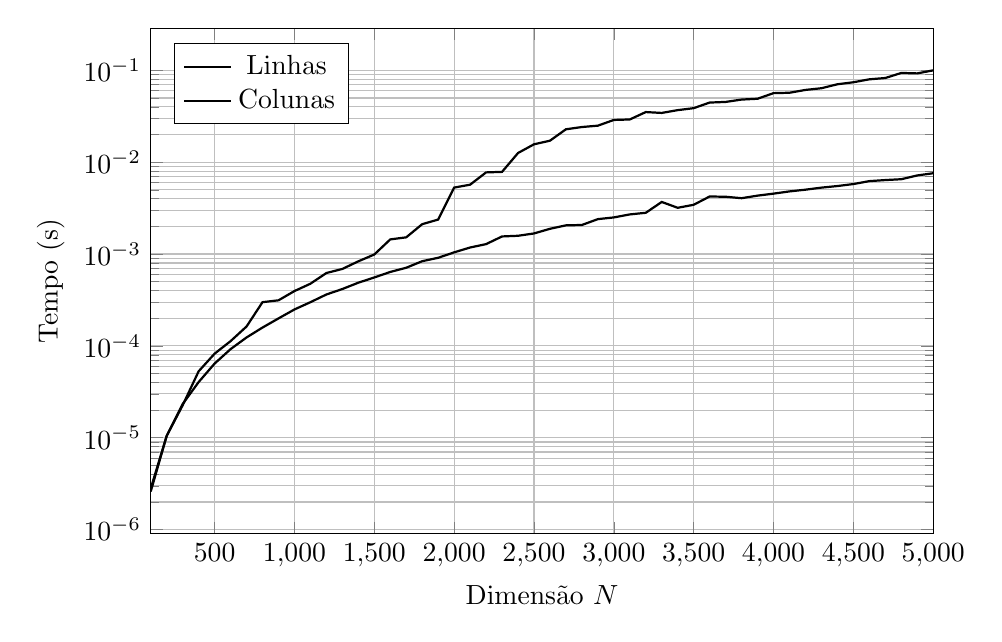
\begin{tikzpicture}

        \begin{semilogyaxis}[
            width=0.95\textwidth,
            height=8cm,
            xlabel={Dimensão \(N\)},
            ylabel={Tempo (s)},
            grid=both,
            legend pos=north west,
            xmin=100,
            xmax=5000
        ]

        \addplot[
            mark=none,
            thick
        ]
        table[row sep=\\] {
            x y\\
            100  0.000002600\\
            200  0.000010500\\
            300  0.000023300\\
            400  0.000040400\\
            500  0.000064250\\
            600  0.000092250\\
            700  0.000123600\\
            800  0.000158450\\
            900  0.000199250\\
            1000 0.000249350\\
            1100 0.000299200\\
            1200 0.000363000\\
            1300 0.000416250\\
            1400 0.000487650\\
            1500 0.000556200\\
            1600 0.000638450\\
            1700 0.000709550\\
            1800 0.000835900\\
            1900 0.000910550\\
            2000 0.001043400\\
            2100 0.001178500\\
            2200 0.001282700\\
            2300 0.001555050\\
            2400 0.001581150\\
            2500 0.001675900\\
            2600 0.001883250\\
            2700 0.002053250\\
            2800 0.002072150\\
            2900 0.002399600\\
            3000 0.002504650\\
            3100 0.002700500\\
            3200 0.002812800\\
            3300 0.003690800\\
            3400 0.003189100\\
            3500 0.003439000\\
            3600 0.004232800\\
            3700 0.004204500\\
            3800 0.004056450\\
            3900 0.004325000\\
            4000 0.004547050\\
            4100 0.004807850\\
            4200 0.005020850\\
            4300 0.005286200\\
            4400 0.005501450\\
            4500 0.005782650\\
            4600 0.006221750\\
            4700 0.006389000\\
            4800 0.006527850\\
            4900 0.007172400\\
            5000 0.007585550\\
        };

        \addlegendentry{Linhas}

        \addplot[
            mark=none,
            thick
        ]
        table[row sep=\\] {
            x y\\
            100  0.000002800\\
            200  0.000010500\\
            300  0.000022600\\
            400  0.000052900\\
            500  0.000082350\\
            600  0.000112700\\
            700  0.000162700\\
            800  0.000299400\\
            900  0.000313600\\
            1000 0.000395500\\
            1100 0.000475400\\
            1200 0.000621800\\
            1300 0.000688600\\
            1400 0.000833400\\
            1500 0.000988800\\
            1600 0.001443650\\
            1700 0.001520900\\
            1800 0.002114750\\
            1900 0.002374200\\
            2000 0.005290200\\
            2100 0.005689650\\
            2200 0.007745000\\
            2300 0.007845800\\
            2400 0.012585500\\
            2500 0.015662600\\
            2600 0.017138500\\
            2700 0.022817450\\
            2800 0.024142200\\
            2900 0.024988600\\
            3000 0.028835600\\
            3100 0.029189850\\
            3200 0.035132500\\
            3300 0.034381000\\
            3400 0.036880900\\
            3500 0.038748050\\
            3600 0.044581250\\
            3700 0.045294700\\
            3800 0.048054400\\
            3900 0.049052650\\
            4000 0.056459450\\
            4100 0.057017050\\
            4200 0.061201900\\
            4300 0.063863850\\
            4400 0.070521800\\
            4500 0.074178500\\
            4600 0.079845450\\
            4700 0.082503350\\
            4800 0.093638850\\
            4900 0.092629950\\
            5000 0.099973250\\
        };

        \addlegendentry{Colunas}

        \end{semilogyaxis}

    \end{tikzpicture}

    \caption{Tempo de execução das implementações por linhas e por colunas.}
    \label{fig:atvd01-tempos}

\end{figure}


\subsection{Evolução da razão C/L}

A Figura~\ref{fig:atvd01-cl} apresenta diretamente a razão entre os tempos.

\begin{figure}[H]
    \centering

    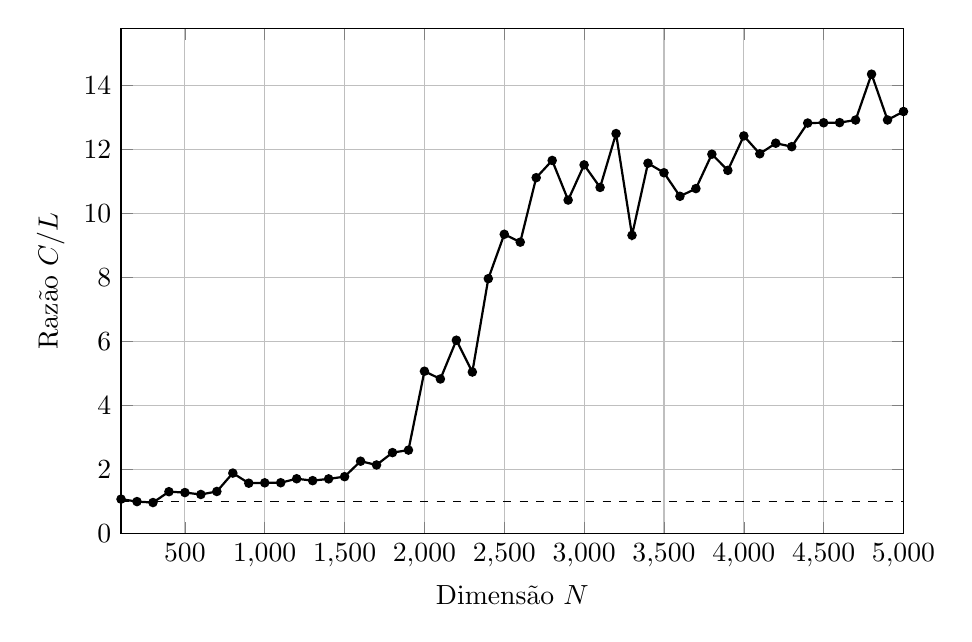
\begin{tikzpicture}

        \begin{axis}[
            width=0.95\textwidth,
            height=8cm,
            xlabel={Dimensão \(N\)},
            ylabel={Razão \(C/L\)},
            grid=both,
            xmin=100,
            xmax=5000,
            ymin=0
        ]

        \addplot[
            mark=*,
            mark size=1.3pt,
            thick
        ]
        table[row sep=\\] {
            x y\\
            100  1.077\\
            200  1.000\\
            300  0.970\\
            400  1.309\\
            500  1.282\\
            600  1.222\\
            700  1.316\\
            800  1.890\\
            900  1.574\\
            1000 1.586\\
            1100 1.589\\
            1200 1.713\\
            1300 1.654\\
            1400 1.709\\
            1500 1.778\\
            1600 2.261\\
            1700 2.143\\
            1800 2.530\\
            1900 2.607\\
            2000 5.070\\
            2100 4.828\\
            2200 6.038\\
            2300 5.045\\
            2400 7.960\\
            2500 9.346\\
            2600 9.100\\
            2700 11.113\\
            2800 11.651\\
            2900 10.414\\
            3000 11.513\\
            3100 10.809\\
            3200 12.490\\
            3300 9.315\\
            3400 11.565\\
            3500 11.267\\
            3600 10.532\\
            3700 10.773\\
            3800 11.846\\
            3900 11.342\\
            4000 12.417\\
            4100 11.859\\
            4200 12.190\\
            4300 12.081\\
            4400 12.819\\
            4500 12.828\\
            4600 12.833\\
            4700 12.913\\
            4800 14.345\\
            4900 12.915\\
            5000 13.179\\
        };

        \addplot[
            dashed
        ]
        coordinates {
            (100,1)
            (5000,1)
        };

        \end{axis}

    \end{tikzpicture}

    \caption{Evolução da razão \(C/L\) em função da dimensão da matriz.}
    \label{fig:atvd01-cl}

\end{figure}


% ============================================================
% DISCUSSÃO
% ============================================================

\section{Análise e discussão}

\label{sec:atvd01-discussao}

\subsection{Região de matrizes pequenas}

Entre \(N=100\) e \(N=700\), os tempos permanecem relativamente próximos.

A mediana da razão \(C/L\) nessa faixa é:

\begin{equation}
    \widetilde{C/L}_{100-700}
    \approx
    1.222.
\end{equation}

Em \(N=200\), por exemplo:

\begin{equation}
    C/L = 1.000.
\end{equation}

Em \(N=300\), foi observado:

\begin{equation}
    C/L = 0.970.
\end{equation}

Esse valor isolado abaixo de 1 não caracteriza uma vantagem estrutural do
percurso por colunas. Os tempos absolutos nessa região são da ordem de
microssegundos e, consequentemente, mais sensíveis ao ruído relativo da
medição.


\subsection{Início da divergência}

Entre \(N=800\) e \(N=1500\), a diferença passa a aparecer de forma mais
regular.

A mediana da razão nessa faixa é aproximadamente:

\begin{equation}
    \widetilde{C/L}_{800-1500}
    \approx
    1.681.
\end{equation}

Em \(N=800\), por exemplo:

\begin{equation}
    C/L = 1.890.
\end{equation}

Essa região pode ser considerada o início experimentalmente observável da
divergência entre os dois padrões de acesso.


\subsection{Divergência consistente}

Entre \(N=1600\) e \(N=1900\), a razão passa a permanecer acima de 2.

Os valores observados foram:

\begin{center}
\begin{tabular}{rr}
\toprule
\(N\) & \(C/L\) \\
\midrule
1600 & 2.261 \\
1700 & 2.143 \\
1800 & 2.530 \\
1900 & 2.607 \\
\bottomrule
\end{tabular}
\end{center}

A mediana da faixa é aproximadamente:

\begin{equation}
    \widetilde{C/L}_{1600-1900}
    \approx
    2.396.
\end{equation}

Nesse ponto, a penalização do percurso por colunas já é consistente e
não depende de um único valor isolado.


\subsection{Mudança expressiva em N=2000}

A transição mais evidente ocorre entre \(N=1900\) e \(N=2000\).

Para \(N=1900\):

\begin{align}
T_{\mathrm{linha}}  &= 0.000910550\ \mathrm{s},\\
T_{\mathrm{coluna}} &= 0.002374200\ \mathrm{s},\\
C/L &= 2.607.
\end{align}

Para \(N=2000\):

\begin{align}
T_{\mathrm{linha}}  &= 0.001043400\ \mathrm{s},\\
T_{\mathrm{coluna}} &= 0.005290200\ \mathrm{s},\\
C/L &= 5.070.
\end{align}

Enquanto o tempo por linhas cresce de forma moderada, o tempo da versão
por colunas mais que dobra nessa transição.

Assim, \(N=2000\) caracteriza uma mudança expressiva no comportamento
experimental.


\subsection{Regime de forte penalização}

Entre \(N=2000\) e \(N=2700\), a mediana de \(C/L\) é aproximadamente:

\begin{equation}
    \widetilde{C/L}_{2000-2700}
    \approx
    6.999.
\end{equation}

Em \(N=2700\):

\begin{equation}
    C/L = 11.113.
\end{equation}

A partir de \(N=2800\), a razão permanece predominantemente na faixa de
aproximadamente 10 a 13.

A mediana obtida entre \(N=2800\) e \(N=5000\) é:

\begin{equation}
    \widetilde{C/L}_{2800-5000}
    \approx
    11.859.
\end{equation}


\subsection{Maior dimensão avaliada}

Para \(N=5000\), foram obtidos:

\begin{align}
T_{\mathrm{linha}}
&=
0.007585550\ \mathrm{s},
\\
T_{\mathrm{coluna}}
&=
0.099973250\ \mathrm{s},
\\
C/L
&=
13.179.
\end{align}

A versão por colunas levou, portanto, aproximadamente 13.18 vezes o tempo
da versão por linhas nesse caso.

Esse resultado ocorre apesar de ambas as implementações permanecerem em
\(O(N^2)\).


\subsection{Relação com o tamanho da matriz}

Como cada elemento possui quatro bytes, o espaço ocupado apenas pela
matriz é:

\begin{equation}
    M(N)
    =
    4N^2
    \quad\text{bytes}.
    \label{eq:atvd01-memoria}
\end{equation}

Alguns pontos relevantes são apresentados na
Tabela~\ref{tab:atvd01-memoria}.

\begin{table}[H]
    \centering

    \caption{Tamanho aproximado da matriz em pontos selecionados.}
    \label{tab:atvd01-memoria}

    \begin{tabular}{rrr}
        \toprule
        \(N\)
        &
        \textbf{Matriz (MiB)}
        &
        \textbf{C/L}
        \\
        \midrule

        200
        & 0.15
        & 1.000
        \\

        1000
        & 3.81
        & 1.586
        \\

        1800
        & 12.36
        & 2.530
        \\

        2000
        & 15.26
        & 5.070
        \\

        3000
        & 34.33
        & 11.513
        \\

        4000
        & 61.04
        & 12.417
        \\

        5000
        & 95.37
        & 13.179
        \\

        \bottomrule
    \end{tabular}

\end{table}


\subsection{Relação com a cache L3}

A cache L3 reportada para a máquina possui:

\begin{equation}
    33792\ \mathrm{KiB}
    =
    33\ \mathrm{MiB}.
\end{equation}

Igualando aproximadamente o tamanho da matriz a essa capacidade:

\begin{equation}
    4N^2
    \approx
    33 \times 1024^2,
\end{equation}

obtém-se:

\begin{equation}
    N
    \approx
    2941.
\end{equation}

De fato:

\begin{align}
M(2900)
&\approx
32.08\ \mathrm{MiB},
\\
M(3000)
&\approx
34.33\ \mathrm{MiB}.
\end{align}

Portanto, a matriz atravessa numericamente a capacidade nominal reportada
da L3 entre \(N=2900\) e \(N=3000\).

Entretanto, a forte divergência entre as versões já aparece em
\(N=2000\), quando a matriz ocupa aproximadamente 15.26 MiB.

Esse resultado é importante porque demonstra que não é adequado explicar
o comportamento simplesmente pela afirmação de que ``a matriz deixou de
caber na L3''.

A capacidade total da cache é apenas um dos fatores envolvidos.

O padrão de acesso por colunas já apresenta:

\begin{equation}
    S_{\mathrm{coluna}}
    =
    8000\ \mathrm{bytes}
\end{equation}

em \(N=2000\), enquanto o percurso por linhas continua utilizando acessos
contíguos de quatro bytes.

Assim, a diferença observada deve ser interpretada principalmente pela
interação entre:

\begin{itemize}

    \item tamanho crescente do conjunto de dados;

    \item baixa localidade espacial do percurso por colunas;

    \item stride crescente;

    \item aproveitamento das linhas de cache;

    \item mecanismos de prefetching;

    \item tradução de endereços;

    \item políticas de substituição da hierarquia de memória.

\end{itemize}


\subsection{Cache L2 reportada}

O sistema reportou 28672 KiB de cache L2, correspondentes a 28 MiB.

Numericamente, uma matriz de inteiros atinge aproximadamente esse volume
em:

\begin{equation}
    N \approx 2709.
\end{equation}

Essa proximidade não deve ser interpretada como evidência de que uma
matriz de aproximadamente 28 MiB esteja integralmente armazenada em uma
única L2 durante o benchmark.

O valor reportado corresponde à capacidade total agregada apresentada
pelo sistema para o processador. Portanto, ele é registrado como
característica do hardware, mas não é utilizado como um limiar causal
direto para a interpretação de uma única thread.


\subsection{Valor máximo de C/L}

O maior valor observado foi:

\begin{equation}
    C/L = 14.345
\end{equation}

em \(N=4800\).

Nesse ponto:

\begin{align}
T_{\mathrm{linha}}
&=
0.006527850\ \mathrm{s},
\\
T_{\mathrm{coluna}}
&=
0.093638850\ \mathrm{s}.
\end{align}

Como em \(N=4900\) e \(N=5000\) a razão retorna para 12.915 e 13.179,
respectivamente, o valor em \(N=4800\) não caracteriza isoladamente uma
nova mudança de regime.

Ele é tratado como uma variação dentro da região de forte penalização já
estabelecida.


% ============================================================
% LIMITAÇÕES
% ============================================================

\section{Limitações e ameaças à validade}

\label{sec:atvd01-limitacoes}

Embora o experimento apresente uma tendência clara, os resultados devem
ser interpretados dentro das seguintes limitações:

\begin{itemize}

    \item o benchmark foi executado em uma única máquina;

    \item os tempos podem sofrer influência do escalonamento do sistema
    operacional e de processos concorrentes;

    \item variações de frequência do processador podem alterar tempos
    absolutos entre execuções;

    \item não foram utilizados contadores de hardware para medir
    diretamente cache misses, TLB misses ou largura de banda;

    \item os tamanhos de cache reportados pelo sistema não representam
    necessariamente a quantidade efetivamente disponível para uma única
    thread durante toda a execução;

    \item mecanismos automáticos de prefetching podem modificar o custo
    de determinados padrões de acesso;

    \item o compilador com \texttt{-O2} pode aplicar transformações que
    afetam os kernels, embora ambas as versões utilizem as mesmas opções;

    \item as menores matrizes apresentam tempos absolutos muito curtos e,
    consequentemente, maior sensibilidade relativa ao overhead e ao ruído;

    \item a inversão da ordem dos laços também modifica o comportamento
    de acesso ao vetor de saída: a versão por linhas acumula em uma
    variável local e grava \texttt{y[i]} uma vez, enquanto a versão por
    colunas realiza atualizações sucessivas no vetor de saída;

    \item o estudo utiliza \texttt{int}; outros tipos de dado alteram o
    tamanho do working set e podem deslocar as regiões de transição.

\end{itemize}

Essas limitações não invalidam a tendência observada, mas impedem atribuir
um ponto específico exclusivamente a um único nível de cache sem medições
microarquiteturais adicionais.


% ============================================================
% CONCLUSÃO
% ============================================================

\section{Conclusões da atividade}

\label{sec:atvd01-conclusao}

O experimento demonstrou que duas implementações com a mesma operação
matemática e a mesma complexidade assintótica podem apresentar
desempenhos substancialmente diferentes em função da ordem de acesso aos
dados.

Para matrizes pequenas, os tempos das duas versões permaneceram próximos.

A partir de aproximadamente \(N=800\), tornou-se possível observar o
início de uma divergência sistemática.

Entre \(N=1600\) e \(N=1900\), a versão por colunas passou a exigir
aproximadamente duas vezes o tempo da versão por linhas.

Em \(N=2000\), a razão alcançou:

\begin{equation}
    C/L = 5.070,
\end{equation}

caracterizando a mudança mais expressiva da região intermediária.

Para matrizes maiores, a penalização aumentou substancialmente. Entre
\(N=2800\) e \(N=5000\), a mediana da razão foi aproximadamente:

\begin{equation}
    C/L = 11.859.
\end{equation}

No maior tamanho avaliado:

\begin{equation}
    C/L = 13.179.
\end{equation}

Os resultados são compatíveis com a diferença entre os padrões de acesso.
O percurso por linhas acompanha a organização row-major e apresenta
elevada localidade espacial. O percurso por colunas utiliza um stride
proporcional a \(N\), reduzindo o aproveitamento imediato dos dados
carregados pela hierarquia de memória.

A atividade também evidencia que a capacidade nominal das caches não
deve ser utilizada isoladamente como explicação. A forte divergência
surge antes de a matriz alcançar a capacidade nominal da L3, indicando
que stride, localidade, prefetching e demais mecanismos da arquitetura
também participam do comportamento observado.

Assim, o principal resultado da atividade pode ser sintetizado pela
seguinte relação:

\begin{equation}
\boxed{
\text{mesmo } O(N^2)
\;\not\Rightarrow\;
\text{mesmo desempenho}
}
\end{equation}

quando os padrões de acesso à memória são diferentes.


% ============================================================
% DEFESA ORAL
% ============================================================

\section{Síntese para defesa oral}

\label{sec:atvd01-defesa}

Os principais pontos para apresentação oral da atividade são:

\begin{enumerate}

    \item \textbf{Problema.}
    Comparar duas implementações da mesma multiplicação matriz-vetor,
    alterando apenas a ordem principal de percurso da matriz.

    \item \textbf{Hipótese.}
    Como a matriz é armazenada em row-major, o percurso por linhas deve
    explorar melhor a localidade espacial do que o percurso por colunas.

    \item \textbf{Complexidade.}
    As duas versões permanecem em \(O(N^2)\). Portanto, a diferença não
    decorre de uma mudança na ordem assintótica do algoritmo.

    \item \textbf{Metodologia.}
    Foram avaliadas matrizes de \(N=100\) até \(N=5000\), em passos de
    100, com uma execução de aquecimento e dez medições por versão. A
    mediana foi utilizada como tempo representativo.

    \item \textbf{Métrica.}
    Foi utilizada a razão
    \(C/L=T_{\mathrm{coluna}}/T_{\mathrm{linha}}\), permitindo interpretar
    diretamente quantas vezes o percurso por colunas foi mais lento.

    \item \textbf{Primeira divergência.}
    A diferença começa a se tornar visível em torno de \(N=800\).

    \item \textbf{Divergência consistente.}
    Entre \(N=1600\) e \(N=1900\), o percurso por colunas apresenta tempo
    aproximadamente duas vezes maior.

    \item \textbf{Mudança mais expressiva.}
    Em \(N=2000\), \(C/L=5.070\).

    \item \textbf{Regime de matrizes grandes.}
    Entre \(N=2800\) e \(N=5000\), a mediana de \(C/L\) foi aproximadamente
    11.859.

    \item \textbf{Maior caso.}
    Para \(N=5000\), a implementação por colunas levou aproximadamente
    13.18 vezes o tempo da implementação por linhas.

    \item \textbf{Explicação arquitetural.}
    Por linhas, o stride principal é de quatro bytes. Por colunas, o
    stride é \(4N\) bytes, atingindo 20.000 bytes em \(N=5000\).

    \item \textbf{Relação com cache.}
    A matriz cruza aproximadamente os 33 MiB nominais da L3 entre
    \(N=2900\) e \(N=3000\), mas a forte divergência já aparece antes.
    Portanto, não é correto atribuir o fenômeno apenas ao instante em que
    a matriz deixa de caber na L3.

    \item \textbf{Conclusão.}
    A atividade evidencia que organização dos dados e localidade de
    memória podem determinar diferenças de desempenho superiores a uma
    ordem de grandeza mesmo quando a complexidade algorítmica permanece
    inalterada.

\end{enumerate}